%%% Uncomment the following for normal slide show
%
%\documentclass[ignorenonframetext]{beamer}

%%% or uncomment this for handouts
%\documentclass[handout,ignorenonframetext]{beamer}

%%% or uncomment this for the article version
\documentclass[11pt]{article}
\usepackage{beamerarticle}
%
\mode<article>
{
  \usepackage{fullpage}
  \usepackage{pgf}
  \usepackage{hyperref}
  \setjobnamebeamerversion{example.beamer}

}
\mode<presentation>
{
  %\usepackage{listings}
  % \usetheme{Dresden}
  % \usetheme{Marburg}
  \usetheme{Hannover}
 % \usetheme{Singapore}
  % \useoutertheme{smoothbars}
  \setbeamercovered{transparent}
 }

\mode<handout>
{
%%% In handout mode give the individual pages a light grey background
\setbeamercolor{background canvas}{bg=black!5}
%%% Put more than one frame on each page to save paper.
\usepackage{pgfpages} 
\pgfpagesuselayout{4 on 1}[letterpaper,border shrink=3mm, landscape]
% \pgfpagesuselayout{2 on 1}[letterpaper,border shrink=5mm, portrait]
% \setbeameroption{show notes}
}
% \usepackage[latin1]{inputenc}

% common pagkages here? 
\usepackage[english]{babel}
\usepackage{listings, float}


\title{The Lambda Calculus}
\author[MM]{Mairead Meagher}
\subject{From "Haskell Programming from First Principles"}

\date{February, 2019}

\begin{document}

\frame{\maketitle}

\section{Introduction}
The lambda calculus is  a model of computation devised in the 1930s by Alonzo Church. A calculus is a method of calculation or reasoning; the lambda calculus is one process for formalising a method.

Functional programming is a computer programming paradigm that relies on functions modelled on mathematical functions. The essence of functional programming is that programs are a combination of expressions. Expressions include concrete values, variables, and also functions. Functions have a more specific definition: they are expressions that are applied to an argument or input, and once applied, can be reduced or evaluated. In Haskell, and in functional programming more generally, functions are first-class: they can be used as values or passed as arguments, or inputs, to yet more functions.

Functional programming languages are all based on the lambda calculus. Some languages in this general category incorporate features into the language that aren’t translatable into lambda expressions. Haskell is a pure functional language, because it does not.

The word purity in functional programming is sometimes also used to mean what is more properly called referential transparency. Referential transparency means that the same function, given the same values to evaluate, will always return the same result in pure functional programming, as they do in mathematics.
Haskell’s pure functional basis also lends it a high degree of abstraction and composability. Abstraction allows you to write shorter, more concise programs by factoring common, repeated structures into more generic code that can be reused.
\section{What is a function?}

If we step back from using the word “lambda,” remember  what a function is. A function is a relation between a set of possible inputs and a set of possible outputs. The function itself defines and represents the relationship. When you apply a function such as addition to two inputs, it maps those two inputs to an output:
\begin{figure} [H]
	\centering
	\includegraphics[page=1,width=.6\textwidth]{../common_images/latexpics}
	\caption{This is not a function}
	\label{fig:relation}
\end{figure}  

\begin{figure} [H]
	\centering
	\includegraphics[page=2,width=.6\textwidth]{../common_images/latexpics}
	\caption{This is a function}
	\label{fig:function}
\end{figure}  
\begin{figure} [H]
	\centering
	\includegraphics[page=3,width=.6\textwidth]{../common_images/latexpics}
	\caption{Function Application}
	\label{fig:funcapp}
\end{figure}  

What matters here is that the relationship of inputs and outputs is defined by the function, and that the output is predictable when you know the input and the function definition.
The following example  defines the relationship. This function is named $f$: \\
\begin{center}
$
f (x) = x+1
$
\end{center}
It is important to understand this structure. 
\section{The structure of lambda terms}

BNF definition of the lambda calculus: \\

\textless $\lambda$-term \textgreater ::= \textless variable \textgreater  \\
$\hspace*{1.2in} $ $|$ $\lambda$ \textless variable \textgreater . \textless $\lambda$-term \textgreater \\
$\hspace*{1.2in} $ $|$ ( \textless $\lambda$-term \textgreater \textless $\lambda$-term \textgreater  ) \\

\textless variable \textgreater ::= $x | y | z | \ldots$ \\ \\
Or, more compactly: \\

$E ::= \ V\  |\  \lambda \  V.E\  |\  (E1\  \ E2) $

$V :: = x \ |\  y\  |\  z\  |\ \ldots $ \\
Where V is an arbitrary variable and $E_{i}$  is an arbitrary $\lambda$-expression.
We call $\lambda$ V the head of the$\lambda$-expression and E the body.

\begin{figure} [H]
	\centering
	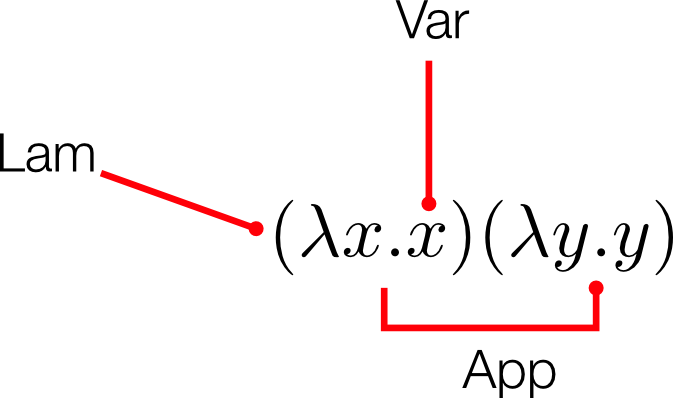
\includegraphics[width=.6\textwidth]{../common_images/lambda}
	\caption{Structure of lambda terms}
	\label{fig:funcapp}
\end{figure}  

The head of the function is a $\lambda$ (lambda) followed by a variable name. The body of the function is another expression. So, a simple function might look like this:
\begin{center}
$\lambda x.x$
\end{center}
The variable named in the head is the parameter and binds all instances of that same variable in the body of the function. That means, when we apply this function to an argument, each $x$ in the body of the function will have the value of that argument. We’ll demonstrate this in the next section.
In the previous section, we were talking about functions called $f$, but the lambda abstraction \begin{center}
$\lambda x.x$
\end{center}
has no name. It is an anonymous function. A named function can be called by name by another function; an anonymous function cannot.

\section{Alpha equivalence}
We have seen the function
\begin{center}
$\lambda x.x$
\end{center}
The variable $x$ here is not semantically meaningful except in its role in that single expression. Because of this, there’s a form of equivalence between lambda terms called alpha equivalence. In other words, 
\begin{center}
$\lambda x.x$ \\
$\lambda apple.apple$\\
$\lambda orange.orange$\\
\end{center}
all mean the same thing. 
\section{Beta reduction}
When we apply a function to an argument, we substitute the input expression for all instances of bound variables within the body of the abstraction. You also eliminate the head of the abstraction, since its only purpose was to bind a variable. This process is called beta reduction.
Let’s use the function we had above:
\begin{center}
$\lambda x.x$
\end{center}
We’ll do our first beta reduction using a number. We apply the function above to 2, substitute 2 for each bound variable in the body of the function, and eliminate the head:
\begin{center}
$(\lambda x.x) \ 2  $ \\
\hspace*{.5in}2
\end{center}
The only bound variable is the single $x$, so applying this function to 2 returns 2. This function is the \textit{identity} function.

Other Examples: 
\begin{center}
$(\lambda x.x+1)$
\end{center}
What happens if we apply this to 2? 
We can also apply our identity function to another lambda abstraction:
\begin{center}
$(\lambda x.x)(\lambda y.y)$
\end{center}

In this case, we substitute the entire abstraction in for $x$. We use a new syntax here, $[x := z]$, to indicate that $z$ will be substituted for all occurrences of $x$ (here $z$ is the function $(\lambda y.y)$). We reduce this application like this:
\begin{center}
$(\lambda x.x)(\lambda y.y)$ \\
$[x  := (\lambda y.y)]$\\
\hspace{.4in}$(\lambda y.y)$\\
\end{center}
Our final result is another identity function. There is no argument to apply it to, so we have nothing to reduce.
Once more, but this time we’ll add another argument:
\begin{center}
$(\lambda x.x)(\lambda y.y)z$
\end{center}

Applications in the lambda calculus are left associative. That is, unless specific parentheses suggest otherwise, they associate, or group, to the left. So, it can be rewritten as:
\begin{center}
$((\lambda x.x)(\lambda y.y)) z$
\end{center}
The $\beta$-reduction is as follows:
\begin{center}
$((\lambda x.x)(\lambda y.y)) z$ \\
\hspace{.22in}$[x := ( \lambda y. y) ] $\\
\hspace{.58in}$ (\lambda y.y) z $ \\
\hspace{.58in}$[y:= z ] $\\
\hspace{1in}$z$ \\
\end{center}
We can't reduce this any further as there is nothing left to apply, and we know nothing about $z$.
\section{Variables}
Variables can be bound or free as the $\lambda$-calculus assumes an infinite universe of free
variables. They are bound to functions in an environment, then they become bound by usage in an abstraction. \\
For example, in the $\lambda$-expression:
\begin{center}
$(\lambda x. x*y)$
\end{center}

x is bound by $\lambda$ over the body $x*y$, but $y$ is a free variable.When we apply this function to an argument, nothing can be done with the $y$. It remains irreducible.
\\
Look at the following when we apply such a function to an argument:  
\begin{center}
$(\lambda x.x*y)z$
\end{center}
We apply the lambda to the argument $z$. \\
\begin{center}
$(\lambda x.x*y)z$ \\
\hspace{.25in}$[x:=z]$ \\
\hspace{.55in}$zy$  \\
\end{center}

The head has been applied away, and there are no more heads or bound variables. Since we know nothing about $z$ or $y$, we can reduce this no further.
\section{Multiple arguments}
Each lambda can only bind one parameter and can only accept one argument. Functions that require multiple arguments have multiple, nested heads. When you apply it once and eliminate the first (leftmost) head, the next one is applied and so on. This means that the following
\begin{center}
$\lambda xy.xy$
\end{center}
is simply syntactic sugar for 
\begin{center}
$\lambda x(\lambda y.xy)$
\end{center}

\section{Syntax trees}
In order to understand the structure of the terms, we look at syntax trees of lambda terms:
\begin{figure} [H]
	\centering
	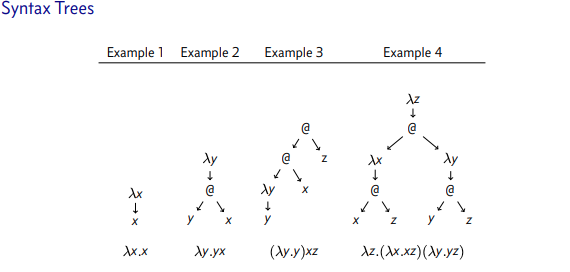
\includegraphics[width=.6\textwidth]{../common_images/syntax-trees}
	\caption{Examples of Syntax trees}
	\label{fig:funcapp}
\end{figure}  
Note that $@$ means function application. 
\begin{figure} [H]
	\centering
	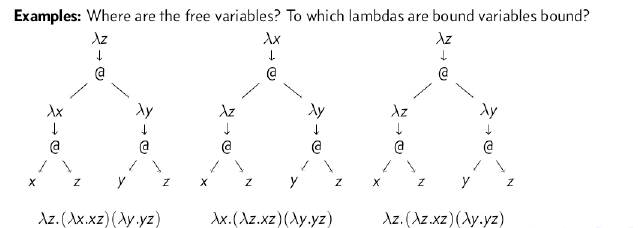
\includegraphics[width=.6\textwidth]{../common_images/free-and-bound}
	\caption{Syntax trees with free and bound variables}
	\label{fig:funcapp}
\end{figure}  
Can you figure which ar the free and bound variables from this diagram? 
 %A well known method of encoding a string in order to disguise its contents is the \textit{Caesar Cipher}
%, named after its use by Julius Caesar. To encode a string, Caesar simple replaced each each letter in the string by the letter places further down in the alphabet. 
%\begin{frame} [fragile, label = test]
%
%  \frametitle{Caesar Cipher}
%
%Example of string encoding with constant shift factor of 3 $\dots$
%    \pause
% \begin{itemize}
% \item
% "abc " would be encoded to "def"  
% \item
% "haskell is fun" would be encoded to "kdnnhoo lv ixq"
%
% \end{itemize}
%
%More Generally 
%\article { the specific shift factor of three used by Caesar can be replaced by any integer between one and twenty-five, thereby giving twenty-five different ways of encoding a string.  So, more generally, with}
%With a shift factor of 4, for example:
%
% \begin{itemize}
% \item
% "abc " would be encoded to "def"  
%  \end{itemize}
%
%How will we use Haskell to implement the Caesar and more \ldots
%\end{frame}
% 
%
%\section{Encoding and decoding}
%We will use a  number of standard functions on characters that are provided in a library called $Data.Char$ which can be loaded into a Haskell script by including the following declaration at the start of the script 
% \begin{frame}[fragile, label=encoding]
%  \frametitle{Encoding and Decoding} 
%   \begin{onlyenv}
%  \begin{lstlisting} [language=Haskell]
% import Data.Char   -- imports standard functions on characters
%  \end{lstlisting}
%  \end{onlyenv}
%
%    \pause
%For simplicity, we will only encode the lower-case characters within a string and leave the other characters unchanged. 
%Firstly 
%\article { $chr$ and $ord$ are Data.Char functions. $chr$ returns a character given its ordinal number. $ord$ returns a given character's ordinal number. }
%  \begin{onlyenv}
%  \begin{lstlisting} [language=Haskell]
%let2Int :: Char -> Int
%let2Int c = ord c - ord 'a' 
%
%int2Let :: Int -> Char
%int2Let n = chr (ord 'a' + n)
% \end{lstlisting}
%  \end{onlyenv}
%We can see them  called in Figure \ref{int2let}
% \begin{figure} 
%
%			\centering
%			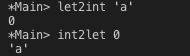
\includegraphics[page=1,width=.5\textwidth]{img/01.png}
%				   \caption{ Calling int2let and let2int}
%		   \label {int2let}
%		   \end{figure}
%
%\end{frame}
%
% \begin{frame}[fragile, label=encoding2]
%  \frametitle{Encoding and Decoding contd. } 
% We define a function \textit{shift} 
% \article {that applies a shift factor to a lower-case letter by converting the letter into the corresponding integer, adding on the shift factor and taking the remainder when divided by 26 (thereby wrapping around the end of the alphabet) and converting the resulting integer back into a lower-case letter. }
% \presentation { as follows: }
% 
%  \begin{itemize}
%  \item   
%  \begin{onlyenv}
%  \begin{lstlisting} [language=Haskell]
%shift :: Int -> Char -> Char
%shift n c   | isLower c = int2let ( 
%                 (let2int c + n ) `mod` 26)
%               | otherwise = c
% \end{lstlisting}
%  \end{onlyenv}    
%  
%  (The library function
%   \begin{onlyenv}
%  \begin{lstlisting} [language=Haskell]
%isLower ::  Char -> Bool
% \end{lstlisting}
%  \end{onlyenv}    
%returns True if it's a lower-case letter.  )
%  \end{itemize}
%  \end{frame}
%
%\begin{frame}[fragile, label=encoding3]
%  \frametitle{Encoding and Decoding contd. } 
%  Using $shift$ within a list comprehension, it is now easy to define a function that encodes a string using a given string factor.
%    \begin{onlyenv}
%  \begin{lstlisting} [language=Haskell]
%encode :: Int -> String -> String 
%encode n xs = [shift n x | x <- xs]
% \end{lstlisting}
%  \end{onlyenv}    
% 
%  We call this as shown in Fig \ref{encode}
%  
%  \begin{figure}
%			\centering
%			
\includegraphics[page=1,width=.5\textwidth]{img/02.png}
%			\caption {Calling encode with positive and negative values}
%			\label{encode}
%		\end{figure}
%\end{frame}
%
%
%\section{Frequency tables}
%
%We now look at cracking the Caesar Cipher. The key to this is the observation that some letters are used more frequently than others in English text. By analysing a large volume of such text one can derive the following table of approximate percentage frequencies of the twenty-six letters of the alphabet : 
%\begin{frame}[fragile, label=freq]
%  \frametitle{Frequency Tables} 
%  \presentation  {Table of approximate percentage frequencies of the twenty-six letters of the alphabet : }
%    \begin{onlyenv}
%  \begin{lstlisting} [language=Haskell]
%table :: [Float]
%table = [8.1, 1.5, 2.8, 4.1, 12.7, 2.2, 2.0, 
%            6.1, 7.0,  0.2, 0.8, 4.0, 2.4, 6.7, 
%            7.5, 1.9, 0.1, 6.0, 6.3, 9.0, 2.8, 
%            1.0, 2.4, 0.2, 2.0, 0.1]
% \end{lstlisting}
% \end{onlyenv}    
%
% \article { For example, the letter 'e' occurs most often, with a frequency of 12.7\% while 'q' and 'z' occur least often with a frequency of just 0.1\%. It is also useful to produce frequency tables for individual strings. To this end, we first define a function that calculates the percentage of  one integer with respect to another, returning the result as a floating point number. This function uses fromIntegral which is a library function converts an integer into a floating point number } 
% \presentation { we define a percent function} 
%     \begin{onlyenv}
%   \begin{lstlisting} [language=Haskell]
%percent :: Int -> Int -> Float
%percent n m = 
%     (fromIntegral n / fromIntegral m ) * 100 
%\end{lstlisting}
%  \end{onlyenv}    
%
%
%\end{frame}
%
%
%\begin{frame}[fragile, label=freq2]
%  \frametitle{Frequency Tables cont. } 
%  We now look at producing a frequency table for a string. We use $count$ and $lowers$ as follows:
%    \begin{onlyenv}
%  \begin{lstlisting} [language=Haskell]
%count :: Eq a => a-> [a] -> Int
%count x xs = length [ x' | x' <- xs, x==x'] 
%
%lowers :: [Char] -> Int
%lowers xs = 
%     length [x| x <- xs, 
%                x >= 'a' && x <= 'z'] 
%\end{lstlisting}
% \end{onlyenv}    
%\end{frame}
%
%
%\begin{frame}[fragile, label=freq3]
%  \frametitle{Frequency Tables cont. } 
%     \begin{onlyenv}
%  \begin{lstlisting} [language=Haskell]
%freqs :: String -> [Float]
%freqs  xs = [percent (count x xs) n | 
%                    x <- ['a'..'z']]
%      where n = lowers xs
%\end{lstlisting}
% \end{onlyenv}    
% 
%  We can see how it's called in Fig \ref{freqs}
%  \begin{figure}
%			\centering
%			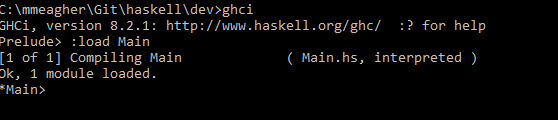
\includegraphics[page=1,width=.5\textwidth]{img/03.png}
%			\caption{Calling freqs on a string}
%			\label{freqs}
%		\end{figure}
%\presentation { the letter 'a' occurs with a frequency of approximately 6.6\%, the letter 'b' with a frequency of 13.3\% etc. }
%\end{frame}
%\article{That is, the letter 'a' occurs with a frequency of approximately 6.6\%, the letter 'b' with a frequency of 13.3\% etc. The use of the $lowers$ function ensures that the percentages are based only on the total number of lower-case letters.}
%\section{Cracking the cipher}
%A standard method for comparing a list of observed frequencies $os$ with a list of expected frequencies $es$ is the \textit{chi-square statistic}, defined by the following summation in which $n$ denotes the length of the two lists. 
%\begin{frame}[fragile, label=freq3]
%  \frametitle{Frequency Tables cont. } 
%  A standard method for comparing 
%  \begin{itemize}
%  \item a list of observed frequencies $os$ with 
%  \item a list of expected frequencies $es$ 
%  \end{itemize}
%  is the \textit{chi-square statistic}, defined by the following summation in which $n$ denotes the length of the two lists. 
%
%\[\sum_{i=0}^{n-1} \frac{(os_i - es_i)^2}{es_i}\]
%\end{frame}
%The smaller the value it produces, the better the match between the two frequency lists.  
%
%\begin{frame} [fragile, label = test]
%  \frametitle{Frequency Tables cont. } 
%  Using $zip$ and list comprehension we translate the previous formula into code
% 
%     \begin{onlyenv}
%  \begin{lstlisting} [language=Haskell]
%chisqr :: [Float] -> [Float] -> Float
%chisqr os es = sum [((o-e)^2)/e | 
%                        (o,e) <- zip os es]
%\end{lstlisting}
% \end{onlyenv}    
% \end{frame}
% 
% \begin{frame} [fragile]
% Now, we define a function that rotates the elements of a list $n$ places the left, wrapping around the start of the list, and assuming that the integer arguments $n$ is between 0 and the $length$ of the list 
%      \begin{onlyenv}
%  \begin{lstlisting} [language=Haskell]
%rotate:: Int -> [a] -> [a]
%rotate n xs = drop n xs ++ take n xs
%\end{lstlisting}
% \end{onlyenv}    
%Now, suppose that we are given an encoded string, but not the shift factor that was used to encode it, and wish to determine this number in order that we can decode the string. This can usually be achieved by producing the frequency table of the encoded string, calculating the chi-square statistic for each possible rotation of the table with respect to the table of expected frequencies, and using the position of the minimum chi-square value as the shift factor. For example, if we let table 
% \end{frame}
% 
% \begin{frame} [fragile]
%     \begin{onlyenv}
%  \begin{lstlisting} [language=Haskell]
%table' = freqs "kdvnhoo lv ixq"
%\end{lstlisting}
% \end{onlyenv}    
%\end{frame}
%
% \begin{frame} [fragile]
%   \begin{onlyenv}
%  \begin{lstlisting} [language=Haskell]
%   [chisqr (rotate' n table') table | n <-  [0..25]]
%   will give us
%   
%    [1409.1558,639.92175,612.2969,
%    202.32024,  1440.2488,  4247.621, 650.89923,  ..]
%\end{lstlisting}
% \end{onlyenv}    
% \end{frame}
% \begin{frame} [fragile]
%
%  \begin{onlyenv}
%  \begin{lstlisting} [language=Haskell]
%crack :: String -> String 
%crack xs = encode (-factor) xs
%    where
%     factor = head (positions  
%     	  ( minimum chitab) chitab ) 
%     chitab = [chisqr (rotate' n table') table | 
%     	      n <- [0..25]]
%     table' = freqs xs
%\end{lstlisting}
% \end{onlyenv}    
%\end{frame}
%%\article {
%%[1409.1558,   639.92175,  612.2969,  202.32024,  1440.2488,  4247.621, 650.89923, 1165.0741, 972.48584, 993.0813, 497.77173, 1490.3737, 2296.2412, 1407.7194, 1491.4241, 3033.884, 659.43945, 2836.2344, 986.21796,  809.58765,   1310.7455, 850.54156, 2907.9312, 954.33203, 5313.4775, 626.3024] }
%%
% \begin{frame} [fragile]
%For example:
%  \begin{onlyenv}
%  \begin{lstlisting} [language=Haskell]
%crack "kdvnhoo lv ixq"
%
%"haskell is fun"
%
%\end{lstlisting}
% \end{onlyenv}    
%\end{frame}
\end{document}
